 \section{Systemarchitektur}
 MongoDB besteht aus drei verschiedenen Servern. Den Routern, Config Servern und
 den Replica Sets. Jeder dieser drei Servertypen hat eine bestimmte Aufgabe.
 Der Client sendet seine Operation an den Router. Der Router wiederum leitet
 die Operation an die zuständigen Replica Sets weiter. Die Replica Sets wiederum 
 speichern die zu verarbeitenden Dokumente. Damit der Router weiss, an welche
 Replica Sets er die Anfrage weiterleiten muss, stellt er wiederum eine Anfrage
 an die Config Server. Diese antworten entsprechend. Die Config Server enthalten 
 also die Metadaten über die Dokumentenverteilung in den Replica Sets.
 In der Abbildung \ref{fig:archmong} ist die Architektur von MongoDB
 visualisiert.
% \begin{figure}[htbp]
% \centering
%    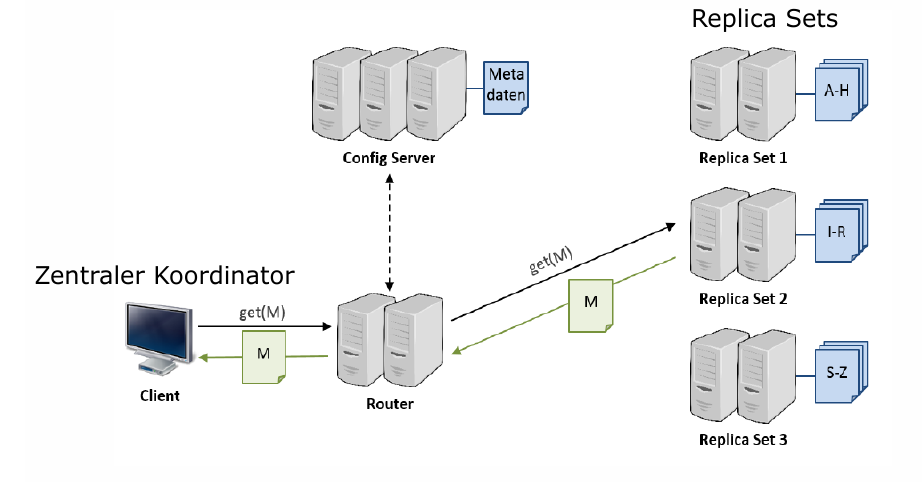
\includegraphics[width=1\textwidth]{./pictures/Architektur_MongoDB.png}
% \caption{Architektur von MongoDB. \cite{Kaufmann2016_DB}}
% \label{fig:archmong}
% \end{figure}
 In der, in diesem Projekt eingesetzte, MongoDB Instanz laufen alle drei Server
 auf demselben physischen Rechner. Dies wurde so gewählt, da die Sammlungen an
 Dokumenten klein sind. Des Weiteren wird auch nur sporadisch auf die Daten
 zugegriffen. Sollte sich in Zukunft einer dieser Parameter ändern, kann darüber
 nachgedacht werden die Server auf verschiedene physische Server zu
 verteilen. Dies hätte auch den weiteren Vorteil, dass parallel auf die
 Dokumente zugegriffen werden könnte. Ist die Replica Set 1 mit der Verarbeitung
 einer Anfrage beschäftigt, kann gleichzeitig die Replica Set 2 die nächste
 Anfrage bearbeiten, sofern es sich bei der Anfrage um die in ihr gespeicherten
 Dokumente handelt. \\\\
 In RDBMS liegen die Tabellen in normalisierter Form vor. Daten die nicht
 funktional vom Primärschlüssel abhängen, werden als Fremdschlüssel
 referenziert. Die Referenzierung macht es schwierig, die Tabelle, in
 welcher das referenzierte Tupel abgelegt ist, auf einen anderen Server
 auszulagern. Denn bei jedem Zugriff auf die ausgelagerte Tabelle wird die
 Abfrage der Daten verlangsamt, da die beiden Server zuerst miteinander kommunizieren müssen. Dieses Problem hat MongoDB nicht, da die Daten nicht normalisiert
 vorliegen müssen. Bei MongoDB dürfen die bei RDBMS referenzierten Tupel als
 Aggretationen in Dokumenten umgesetzt werden. Dies vermindert die Anzahl der
 Referenzierungen und ermöglicht es damit, dass eine horizontale Skalierung
 einfacher zu bewerkstelligen ist, als bei einer relationalen Datenbank. Dies
 führt aber auch Nachteile mit sich. Jedes mal wenn ein referenziertes
 Tupel als Aggregation in ein Dokument gespeichert wird, erhöht sich die
 Datenmenge. Des Weiteren bedeutet es mehr Aufwand, ein solches aggregiertes
 Tupel zu ändern, da die Änderung bei allen Dokumenten gemacht werden muss, bei denen
 das referenzierte Tupel als Unterteil gespeichert wurde. Dies im Gegensatz zur
 relationalen Datenbank. Bei dieser muss die Änderung nur an einem Ort
 stattfinden. MongoDB kennt keine Funktionalität zum Auflösen von Referenzen, diese muss jeweils in der Applikation implementiert werden. \\\\
 Da wie bereits erwähnt, alle Server auf einem physischen Rechner
 laufen, ist die Datenbank bei einem Systemausfall nicht mehr erreichbar.
 Bei einem Festplattenausfall kann es sogar passieren, dass die komplette
 Datenbank verloren geht, da es in der Replica Set nur einen Server gibt, und
 somit ein weiter Server fehlt, der ein Replikat der Datenbank enthält.
 